% vim: set spell spelllang=en tw=100 et sw=4 sts=4 foldmethod=marker foldmarker={{{,}}} :

\documentclass{beamer}

\usepackage{tikz}
\usepackage{xcolor}
\usepackage{complexity}
\usepackage{hyperref}
\usepackage{microtype}
\usepackage{amsmath}                   % \operatorname
\usepackage{amsfonts}                  % \mathcal
\usepackage{amssymb}                   % \nexists
\usepackage{gnuplot-lua-tikz}          % graphs
\usepackage[vlined]{algorithm2e} % algorithms
\usepackage{centernot}

\usetikzlibrary{shapes, arrows, shadows, calc, positioning, fit}
\usetikzlibrary{decorations.pathreplacing, decorations.pathmorphing, shapes.misc}
\usetikzlibrary{tikzmark}

\definecolor{uofguniversityblue}{rgb}{0, 0.219608, 0.396078}

\definecolor{uofgheather}{rgb}{0.356863, 0.32549, 0.490196}
\definecolor{uofgaquamarine}{rgb}{0.603922, 0.72549, 0.678431}
\definecolor{uofgslate}{rgb}{0.309804, 0.34902, 0.380392}
\definecolor{uofgrose}{rgb}{0.823529, 0.470588, 0.709804}
\definecolor{uofgmocha}{rgb}{0.709804, 0.564706, 0.47451}
\definecolor{uofgsandstone}{rgb}{0.321569, 0.278431, 0.231373}
\definecolor{uofgforest}{rgb}{0, 0.2, 0.129412}
\definecolor{uofglawn}{rgb}{0.517647, 0.741176, 0}
\definecolor{uofgcobalt}{rgb}{0, 0.615686, 0.92549}
\definecolor{uofgturquoise}{rgb}{0, 0.709804, 0.819608}
\definecolor{uofgsunshine}{rgb}{1.0, 0.862745, 0.211765}
\definecolor{uofgpumpkin}{rgb}{1.0, 0.72549, 0.282353}
\definecolor{uofgthistle}{rgb}{0.584314, 0.070588, 0.447059}
\definecolor{uofgrust}{rgb}{0.603922, 0.227451, 0.023529}
\definecolor{uofgburgundy}{rgb}{0.490196, 0.133333, 0.223529}
\definecolor{uofgpillarbox}{rgb}{0.701961, 0.047059, 0}
\definecolor{uofglavendar}{rgb}{0.356863, 0.301961, 0.580392}

\tikzset{vertex/.style={draw, circle, inner sep=0pt, minimum size=0.5cm, font=\small\bfseries}}
\tikzset{notvertex/.style={vertex, color=white, text=black}}
\tikzset{plainvertex/.style={vertex}}
\tikzset{vertexc1/.style={vertex, fill=uofgburgundy, text=white}}
\tikzset{vertexc2/.style={vertex, fill=uofgsandstone, text=white}}
\tikzset{vertexc3/.style={vertex, fill=uofgforest, text=white}}
\tikzset{vertexc4/.style={vertex, fill=uofgheather, text=white}}
\tikzset{edge/.style={color=black!50!white}}
\tikzset{bedge/.style={ultra thick}}

% {{{ theme things
\useoutertheme[footline=authortitle]{miniframes}
\useinnertheme{rectangles}

\setbeamerfont{block title}{size={}}
\setbeamerfont{title}{size=\large,series=\bfseries}
\setbeamerfont{section title}{size=\large,series=\mdseries}
\setbeamerfont{author}{size=\normalsize,series=\mdseries}
\setbeamercolor*{structure}{fg=uofguniversityblue}
\setbeamercolor*{palette primary}{use=structure,fg=black,bg=white}
\setbeamercolor*{palette secondary}{use=structure,fg=white,bg=uofgcobalt}
\setbeamercolor*{palette tertiary}{use=structure,fg=white,bg=uofguniversityblue}
\setbeamercolor*{palette quaternary}{fg=white,bg=black}

\setbeamercolor*{titlelike}{parent=palette primary}

\beamertemplatenavigationsymbolsempty

\setbeamertemplate{title page}
{
    \begin{tikzpicture}[remember picture, overlay]
        \node at (current page.north west) {
            \begin{tikzpicture}[remember picture, overlay]
                \fill [fill=white, anchor=north west, yshift=-0.5cm, opacity=0.8] (0, 0) rectangle (\paperwidth, -3.2cm);
            \end{tikzpicture}
        };

        \node at (current page.north west) {
            \begin{tikzpicture}[remember picture, overlay]
                \fill [fill=white, anchor=north west, yshift=-0.5cm, xshift=0.7\paperwidth] (0, 0) rectangle (0.3\paperwidth, -3.2cm);
            \end{tikzpicture}
        };

        \node (logo) [anchor=north east, shift={(-0.15cm,-0.65cm)}] at (current page.north east) {
            \begin{minipage}{0.25\paperwidth}
                \begin{center}
                \includegraphics*[keepaspectratio=true,scale=0.45]{UoG_colour.pdf} \\[0.15cm]
                    \colorbox{white}{\includegraphics*[keepaspectratio=true,scale=0.14]{Universite_Lyon_1.pdf}}\\[0.15cm]
                \includegraphics*[keepaspectratio=true,scale=0.12]{Logo_INSALyon-pantone-cartouche.pdf}
                \end{center}
            \end{minipage}
        };

        \node [anchor=west, xshift=0.1cm] at (current page.west |- logo.west) {
            \begin{minipage}{0.70\paperwidth}\raggedright
                {\usebeamerfont{title}\usebeamercolor[black]{}\inserttitle}\\[0.2cm]
                {\usebeamerfont{author}\usebeamercolor[black]{}\insertauthor}
            \end{minipage}
        };
    \end{tikzpicture}
}

\setbeamertemplate{section page}
{
    \begin{centering}
        \begin{beamercolorbox}[sep=12pt,center]{part title}
            \usebeamerfont{section title}\insertsection\par
        \end{beamercolorbox}
    \end{centering}
}

\newcommand{\frameofframes}{/}
\newcommand{\setframeofframes}[1]{\renewcommand{\frameofframes}{#1}}

\makeatletter
\setbeamertemplate{footline}
{%
    \begin{beamercolorbox}[colsep=1.5pt]{upper separation line foot}
    \end{beamercolorbox}
    \begin{beamercolorbox}[ht=2.5ex,dp=1.125ex,%
        leftskip=.3cm,rightskip=.3cm plus1fil]{author in head/foot}%
        \leavevmode{\usebeamerfont{author in head/foot}\insertshortauthor}%
        \hfill%
        {\usebeamerfont{institute in head/foot}\usebeamercolor[fg]{institute in head/foot}\insertshortinstitute}%
    \end{beamercolorbox}%
    \begin{beamercolorbox}[ht=2.5ex,dp=1.125ex,%
        leftskip=.3cm,rightskip=.3cm plus1fil]{title in head/foot}%
        {\usebeamerfont{title in head/foot}\insertshorttitle}%
        \hfill%
        {\usebeamerfont{frame number}\usebeamercolor[fg]{frame number}\insertframenumber~\frameofframes~\inserttotalframenumber}
    \end{beamercolorbox}%
    \begin{beamercolorbox}[colsep=1.5pt]{lower separation line foot}
    \end{beamercolorbox}
}

\makeatletter
\newenvironment{nearlyplainframe}[2][]{
    \def\beamer@entrycode{\vspace*{-\headheight}\vspace*{3pt}}
    \setbeamertemplate{headline}
    {%
        \begin{beamercolorbox}[colsep=1.5pt]{upper separation line head}
        \end{beamercolorbox}
        \begin{beamercolorbox}[ht=0.5ex,dp=0.125ex,%
            leftskip=.3cm,rightskip=.3cm plus1fil]{title in head/foot}%
        \end{beamercolorbox}%
        \begin{beamercolorbox}[ht=0.5ex,dp=0.125ex,%
            leftskip=.3cm,rightskip=.3cm plus1fil]{author in head/foot}%
        \end{beamercolorbox}%
        \begin{beamercolorbox}[colsep=1.5pt]{lower separation line head}
        \end{beamercolorbox}
        \vspace*{\headheight}
    }

    \setbeamertemplate{footline}
    {%
        \begin{beamercolorbox}[colsep=1.5pt]{upper separation line foot}
        \end{beamercolorbox}
        \begin{beamercolorbox}[ht=0.5ex,dp=0.125ex,%
            leftskip=.3cm,rightskip=.3cm plus1fil]{author in head/foot}%
        \end{beamercolorbox}%
        \begin{beamercolorbox}[ht=0.5ex,dp=0.125ex,%
            leftskip=.3cm,rightskip=.3cm plus1fil]{title in head/foot}%
        \end{beamercolorbox}%
        \begin{beamercolorbox}[colsep=1.5pt]{lower separation line foot}
        \end{beamercolorbox}
    }

    \begin{frame}[#1]{#2}
    }{
    \end{frame}
}
\makeatother

% }}}

\author[Ciaran McCreesh, Samba Ndojh Ndiaye, Patrick Prosser and Christine Solnon]{Ciaran McCreesh,
Samba Ndojh Ndiaye, \\ Patrick Prosser and Christine Solnon}
\title{Clique and Constraint Models for Maximum Common (Connected) Subgraph Problems}

\begin{document}

{
    \usebackgroundtemplate{
        \tikz[overlay, remember picture]
        \node[at=(current page.south), anchor=south, inner sep=0pt]{\includegraphics*[keepaspectratio=true, height=\paperheight]{background.jpg}};
    }
    \begin{frame}[plain,noframenumbering]
        \titlepage
    \end{frame}
}

\begin{frame}{Maximum Common Induced Subgraph}
    \centering
    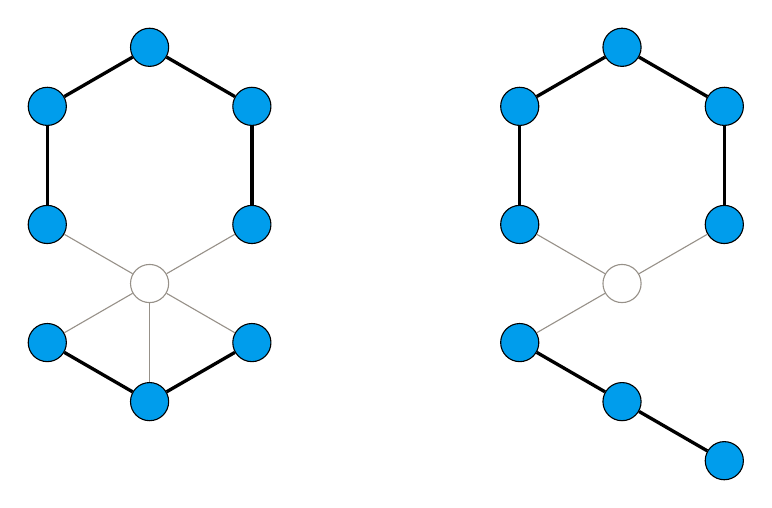
\begin{tikzpicture}
        \begin{scope}
            \node[draw, circle, fill=uofgcobalt, inner sep=2pt, font=\normalsize] (M1) at (90:1.5) {\phantom{0}};
            \node[draw, circle, fill=uofgcobalt, inner sep=2pt, font=\normalsize] (M2) at (150:1.5) {\phantom{0}};
            \node[draw, circle, fill=uofgcobalt, inner sep=2pt, font=\normalsize] (M3) at (30:1.5) {\phantom{0}};
            \node[draw, circle, fill=uofgcobalt, inner sep=2pt, font=\normalsize] (M4) at (210:1.5) {\phantom{0}};
            \node[draw, circle, fill=uofgcobalt, inner sep=2pt, font=\normalsize] (M5) at (330:1.5) {\phantom{0}};
            \node[draw, circle, draw=uofgsandstone!60, fill=white, inner sep=2pt, font=\normalsize] (M6) at (270:1.5) {\phantom{0}};
            \node[draw, circle, fill=uofgcobalt, inner sep=2pt, font=\normalsize] (M7) at ($(210:1.5) + (M6)$) {\phantom{0}};
            \node[draw, circle, fill=uofgcobalt, inner sep=2pt, font=\normalsize] (M8) at ($(330:1.5) + (M6)$) {\phantom{0}};
            \node[draw, circle, fill=uofgcobalt, inner sep=2pt, font=\normalsize] (M9) at ($(270:1.5) + (M6)$) {\phantom{0}};

            \draw [very thick] (M1) -- (M2);
            \draw [very thick] (M2) -- (M4);
            \draw [very thick] (M3) -- (M5);
            \draw [color=uofgsandstone!60] (M4) -- (M6);
            \draw [color=uofgsandstone!60] (M5) -- (M6);
            \draw [very thick] (M3) -- (M1);
            \draw [color=uofgsandstone!60] (M6) -- (M7);
            \draw [color=uofgsandstone!60] (M6) -- (M8);
            \draw [color=uofgsandstone!60] (M6) -- (M9);
            \draw [very thick] (M7) -- (M9);
            \draw [very thick] (M8) -- (M9);
        \end{scope}

        \begin{scope}[xshift=6cm]
            \node[draw, circle, fill=uofgcobalt, inner sep=2pt, font=\normalsize] (M1) at (90:1.5) {\phantom{0}};
            \node[draw, circle, fill=uofgcobalt, inner sep=2pt, font=\normalsize] (M2) at (150:1.5) {\phantom{0}};
            \node[draw, circle, fill=uofgcobalt, inner sep=2pt, font=\normalsize] (M3) at (30:1.5) {\phantom{0}};
            \node[draw, circle, fill=uofgcobalt, inner sep=2pt, font=\normalsize] (M4) at (210:1.5) {\phantom{0}};
            \node[draw, circle, fill=uofgcobalt, inner sep=2pt, font=\normalsize] (M5) at (330:1.5) {\phantom{0}};
            \node[draw, circle, draw=uofgsandstone!60, fill=white, inner sep=2pt, font=\normalsize] (M6) at (270:1.5) {\phantom{0}};
            \node[draw, circle, fill=uofgcobalt, inner sep=2pt, font=\normalsize] (M7) at ($(210:1.5) + (M6)$) {\phantom{0}};
            \node[draw, circle, fill=uofgcobalt, inner sep=2pt, font=\normalsize] (M8) at ($(270:1.5) + (M6)$) {\phantom{0}};
            \node[draw, circle, fill=uofgcobalt, inner sep=2pt, font=\normalsize] (M9) at ($(330:1.5) + (M8)$) {\phantom{0}};

            \draw [very thick] (M1) -- (M2);
            \draw [very thick] (M2) -- (M4);
            \draw [very thick] (M3) -- (M5);
            \draw [color=uofgsandstone!60] (M4) -- (M6);
            \draw [color=uofgsandstone!60] (M5) -- (M6);
            \draw [very thick] (M3) -- (M1);
            \draw [color=uofgsandstone!60] (M6) -- (M7);
            \draw [very thick] (M7) -- (M8);
            \draw [very thick] (M8) -- (M9);
        \end{scope}
    \end{tikzpicture}
\end{frame}

\begin{frame}{Why Care?}
    \begin{itemize}
        \item To determine the similarity between two graphs.
            \begin{itemize}
                \item Edit distance comes down to what's not in the maximum common subgraph.
            \end{itemize}

        \item As a relaxed form of subgraph isomorphism.
    \end{itemize}
\end{frame}

\begin{frame}{CP Models}
    \begin{itemize}
        \item One variable for each vertex in the smaller input graph.
        \item Domains range over vertices in the other input graph, plus $\bot$.
        \item Objective is to maximise variables not assigned $\bot$.
        \item Adjacent pairs of non-$\bot$ vertices must be mapped to adjacent pairs of vertices.
        \item Non-adjacent pairs of non-$\bot$ vertices must be mapped to non-adjacent pairs of vertices.
        \item All different except $\bot$, with number of allowed $\bot$ occurrences controlled by
            the objective variable.
        \item Smallest domain first, prefer vertices of similar degree.
    \end{itemize}
\end{frame}

\begin{frame}{Clique Models and Microstructure}
    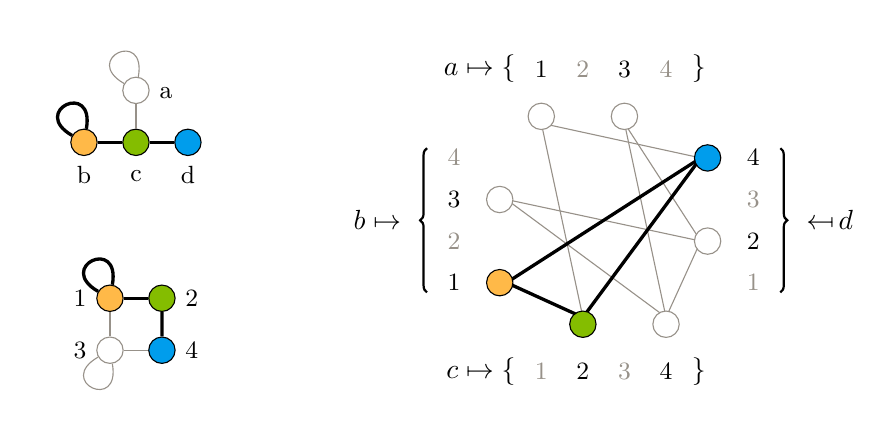
\begin{tikzpicture}[scale=0.33]%{{{
        \begin{scope}
            \node[draw, circle, fill=white, draw=uofgsandstone!60, inner sep=0.5pt, font=\normalsize] (Ma) at (2, 8) {\phantom{0}};
            \node[draw, circle, fill=uofgpumpkin, inner sep=0.5pt, font=\normalsize] (Mb) at (0, 6) {\phantom{0}};
            \node[draw, circle, fill=uofglawn, inner sep=0.5pt, font=\normalsize] (Mc) at (2, 6) {\phantom{0}};
            \node[draw, circle, fill=uofgcobalt, inner sep=0.5pt, font=\normalsize] (Md) at (4, 6) {\phantom{0}};

            \node [right = 0 of Ma, font=\small] { \vphantom{0}a };
            \node [below = 0 of Mb, font=\small] { \vphantom{0}b };
            \node [below = 0 of Mc, font=\small] { \vphantom{0}c };
            \node [below = 0 of Md, font=\small] { \vphantom{0}d };

            \draw [very thick] (Mb) -- (Mc);
            \draw [very thick] (Mc) -- (Md);
            \draw [color=uofgsandstone!60] (Ma) -- (Mc);
            \draw [color=uofgsandstone!60] (Ma) to [out=150, in=80, looseness=8] (Ma);
            \draw [very thick] (Mb) to [out=150, in=80, looseness=8] (Mb);
        \end{scope}

        \begin{scope}[yshift=-2cm]
            \node[draw, circle, fill=uofgpumpkin, inner sep=0.5pt, font=\normalsize] (M1) at (1, 2) {\phantom{0}};
            \node[draw, circle, fill=uofglawn, inner sep=0.5pt, font=\normalsize] (M2) at (3, 2) {\phantom{0}};
            \node[draw, circle, fill=white, draw=uofgsandstone!60, inner sep=0.5pt, font=\normalsize] (M3) at (1, 0) {\phantom{0}};
            \node[draw, circle, fill=uofgcobalt, inner sep=0.5pt, font=\normalsize] (M4) at (3, 0) {\phantom{0}};

            \node [left = 0 of M1, font=\small] { \vphantom{0}1 };
            \node [right = 0 of M2, font=\small] { \vphantom{0}2 };
            \node [left = 0 of M3, font=\small] { \vphantom{0}3 };
            \node [right = 0 of M4, font=\small] { \vphantom{0}4 };

            \draw [very thick] (M1) -- (M2);
            \draw [very thick] (M2) -- (M4);
            \draw [color=uofgsandstone!60] (M3) -- (M4);
            \draw [color=uofgsandstone!60] (M1) -- (M3);

            \draw [color=uofgsandstone!60] (M3) to [out=280, in=210, looseness=8] (M3);
            \draw [very thick] (M1) to [out=150, in=80, looseness=8] (M1);
        \end{scope}

        \begin{scope}[xshift=15cm, yshift=-2cm]
            \node[draw, circle, fill=white, draw=uofgsandstone!60, inner sep=0.5pt, font=\normalsize] (Ma1) at (2.6, 9) {\phantom{0}};
            \node[draw, circle, fill=white, draw=white, inner sep=0.5pt, font=\normalsize] (Ma2) at (4.2, 9) {\phantom{0}};
            \node[draw, circle, fill=white, draw=uofgsandstone!60, inner sep=0.5pt, font=\normalsize] (Ma3) at (5.8, 9) {\phantom{0}};
            \node[draw, circle, fill=white, draw=white, inner sep=0.5pt, font=\normalsize] (Ma4) at (7.4, 9) {\phantom{0}};
            \node (La1) [above = 0.2cm of Ma1, font=\small] { \vphantom{0}1 };
            \node (La2) [above = 0.2cm of Ma2, font=\small, color=uofgsandstone!60] { \vphantom{0}2 };
            \node (La3) [above = 0.2cm of Ma3, font=\small] { \vphantom{0}3 };
            \node (La4) [above = 0.2cm of Ma4, font=\small, color=uofgsandstone!60] { \vphantom{0}4 };

            \node [left=0 of La1] { $a \mapsto \{$ };
            \node [right=0 of La4] { $\}$ };

            \node[draw, circle, fill=uofgpumpkin, inner sep=0.5pt, font=\normalsize] (Mb1) at (1, 2.6) {\phantom{0}};
            \node[draw, circle, fill=white, draw=white, inner sep=0.5pt, font=\normalsize] (Mb2) at (1, 4.2) {\phantom{0}};
            \node[draw, circle, fill=white, draw=uofgsandstone!60, inner sep=0.5pt, font=\normalsize] (Mb3) at (1, 5.8) {\phantom{0}};
            \node[draw, circle, fill=white, draw=white, inner sep=0.5pt, font=\normalsize] (Mb4) at (1, 7.4) {\phantom{0}};
            \node [left = 0.2cm of Mb1, font=\small] { \vphantom{0}1 };
            \node [left = 0.2cm of Mb2, font=\small, color=uofgsandstone!60] { \vphantom{0}2 };
            \node [left = 0.2cm of Mb3, font=\small] { \vphantom{0}3 };
            \node [left = 0.2cm of Mb4, font=\small, color=uofgsandstone!60] { \vphantom{0}4 };

            \draw [decorate, decoration={brace, raise=0.8cm}, thick] (Mb1.south west) -- (Mb4.north west) node [midway, left=1cm] { $b \mapsto$ };

            \node[draw, circle, fill=white, draw=white, inner sep=0.5pt, font=\normalsize] (Mc1) at (2.6, 1) {\phantom{0}};
            \node[draw, circle, fill=uofglawn, inner sep=0.5pt, font=\normalsize] (Mc2) at (4.2, 1) {\phantom{0}};
            \node[draw, circle, fill=white, draw=white, inner sep=0.5pt, font=\normalsize] (Mc3) at (5.8, 1) {\phantom{0}};
            \node[draw, circle, fill=white, draw=uofgsandstone!60, inner sep=0.5pt, font=\normalsize] (Mc4) at (7.4, 1) {\phantom{0}};
            \node (Lc1) [below = 0.2cm of Mc1, font=\small, color=uofgsandstone!60] { \vphantom{0}1 };
            \node (Lc2) [below = 0.2cm of Mc2, font=\small] { \vphantom{0}2 };
            \node (Lc3) [below = 0.2cm of Mc3, font=\small, color=uofgsandstone!60] { \vphantom{0}3 };
            \node (Lc4) [below = 0.2cm of Mc4, font=\small] { \vphantom{0}4 };

            \node [left=0 of Lc1] { $c \mapsto \{$ };
            \node [right=0 of Lc4] { $\}$ };

            \node[draw, circle, fill=white, draw=white, inner sep=0.5pt, font=\normalsize] (Md1) at (9, 2.6) {\phantom{0}};
            \node[draw, circle, fill=white, draw=uofgsandstone!60, inner sep=0.5pt, font=\normalsize] (Md2) at (9, 4.2) {\phantom{0}};
            \node[draw, circle, fill=white, draw=white, inner sep=0.5pt, font=\normalsize] (Md3) at (9, 5.8) {\phantom{0}};
            \node[draw, circle, fill=uofgcobalt, inner sep=0.5pt, font=\normalsize] (Md4) at (9, 7.4) {\phantom{0}};
            \node [right = 0.2cm of Md1, font=\small, color=uofgsandstone!60] { \vphantom{0}1 };
            \node [right = 0.2cm of Md2, font=\small] { \vphantom{0}2 };
            \node [right = 0.2cm of Md3, font=\small, color=uofgsandstone!60] { \vphantom{0}3 };
            \node [right = 0.2cm of Md4, font=\small] { \vphantom{0}4 };

            \draw [decorate, decoration={brace, raise=0.8cm}, thick] (Md4.north east) -- (Md1.south east) node [midway, right=1cm] { $\reflectbox{\ensuremath{\mapsto}}\, d$ };

            \begin{scope}[on background layer]
                \draw [draw=uofgsandstone!60] ($(Ma1.south)!0.5!(Ma1)$) -- ($(Md4.west)!0.5!(Md4)$);
                \draw [draw=uofgsandstone!60] ($(Ma1.south)!0.5!(Ma1)$) -- ($(Mc2.north)!0.5!(Mc2)$);
                \draw [draw=uofgsandstone!60] ($(Ma3.south)!0.5!(Ma3)$) -- ($(Mc4.north)!0.5!(Mc4)$);
                \draw [draw=uofgsandstone!60] ($(Mb3.east)!0.5!(Mb3)$) -- ($(Mc4.north)!0.5!(Mc4)$);
                \draw [draw=uofgsandstone!60] ($(Md2.west)!0.5!(Md2)$) -- ($(Mc4.north)!0.5!(Mc4)$);
                \draw [draw=uofgsandstone!60] ($(Md2.west)!0.5!(Md2)$) -- ($(Ma3.south)!0.5!(Ma3)$);
                \draw [draw=uofgsandstone!60] ($(Md2.west)!0.5!(Md2)$) -- ($(Mb3.east)!0.5!(Mb3)$);
                \draw [very thick] ($(Mb1.east)!0.5!(Mb1)$) -- ($(Mc2.north)!0.5!(Mc2)$);
                \draw [very thick] ($(Mb1.east)!0.5!(Mb1)$) -- ($(Md4.west)!0.5!(Md4)$);
                \draw [very thick] ($(Mc2.north)!0.5!(Mc2)$) -- ($(Md4.west)!0.5!(Md4)$);
        \end{scope}
        \end{scope}

    \end{tikzpicture}
\end{frame}

\begin{frame}{Benchmark Instances}
    \begin{itemize}
        \item Standard benchmark suite of 81,000 instances (random with varying densities; 2D, 3D
            and 4D regular and irregular meshes; regular bounded degree graphs, and irregular
            bounded degree graphs).
        \item Unlabelled:
            \begin{itemize}
                \item Up to 35 vertices.
            \end{itemize}
        \item Labels on vertices and edges:
            \begin{itemize}
                \item Up to 100 vertices.
                \item Number of labels is 33\% of the number of vertices.
            \end{itemize}
    \end{itemize}
\end{frame}

\begin{frame}{Conventional Wisdom}
    \begin{itemize}
        \item We all know that microstructure is only of theoretical interest, and that solving CSPs
            by reduction is a silly idea.
        \item Several papers say the clique encoding is terrible.
            \begin{itemize}
                \item But this is based upon benchmarking against either maximal clique enumeration
                    algorithms, or very simple maximum clique algorithms.
            \end{itemize}
    \end{itemize}
\end{frame}

\begin{nearlyplainframe}[t]{So Which is Better?}
    \only<1>{
        \begin{center}
            \includegraphics*{gen-graph-unconnected-cumulative-unlabelled.pdf}
        \end{center}
    }

    \only<2>{
        \begin{center}
            \includegraphics*{gen-graph-unconnected-heatmap-unlabelled.pdf}
        \end{center}
    }

    \only<3>{
        \begin{center}
            \includegraphics*{gen-graph-unconnected-cumulative-labelled.pdf}
        \end{center}
    }

    \only<4>{
        \begin{center}
            \includegraphics*{gen-graph-unconnected-heatmap-labelled.pdf}
        \end{center}
    }
\end{nearlyplainframe}

\begin{frame}{Why?}
    \begin{itemize}
        \item Vertex labels:
            \begin{itemize}
                \item Remove values from domains in the CP encoding.
                \item Remove vertices in the clique encoding.
            \end{itemize}
        \item Edge labels:
            \begin{itemize}
                \item Don't do anything for MAC so long as $\bot$ remains in domains.

                \item Remove edges in the clique encoding. Maximum clique algorithms like sparse
                    graphs.
            \end{itemize}
    \end{itemize}
\end{frame}

\begin{frame}{Are We Solving the Right Problem?}
    \centering
    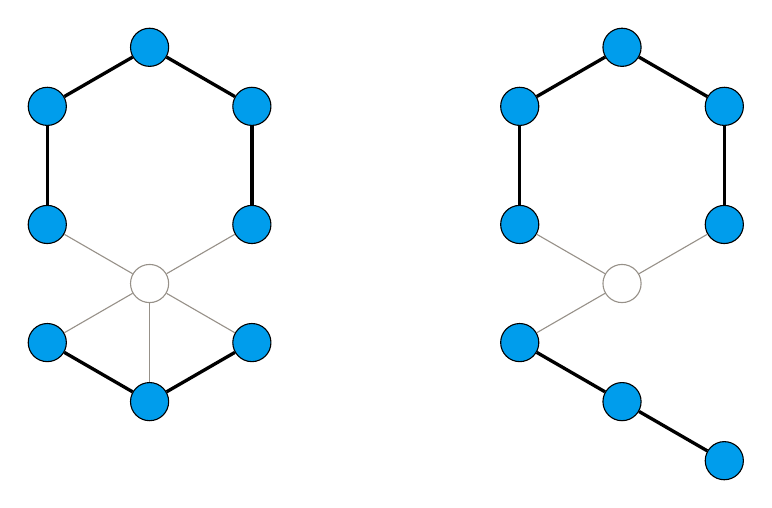
\begin{tikzpicture}
        \begin{scope}
            \node[draw, circle, fill=uofgcobalt, inner sep=2pt, font=\normalsize] (M1) at (90:1.5) {\phantom{0}};
            \node[draw, circle, fill=uofgcobalt, inner sep=2pt, font=\normalsize] (M2) at (150:1.5) {\phantom{0}};
            \node[draw, circle, fill=uofgcobalt, inner sep=2pt, font=\normalsize] (M3) at (30:1.5) {\phantom{0}};
            \node[draw, circle, fill=uofgcobalt, inner sep=2pt, font=\normalsize] (M4) at (210:1.5) {\phantom{0}};
            \node[draw, circle, fill=uofgcobalt, inner sep=2pt, font=\normalsize] (M5) at (330:1.5) {\phantom{0}};
            \node[draw, circle, draw=uofgsandstone!60, fill=white, inner sep=2pt, font=\normalsize] (M6) at (270:1.5) {\phantom{0}};
            \node[draw, circle, fill=uofgcobalt, inner sep=2pt, font=\normalsize] (M7) at ($(210:1.5) + (M6)$) {\phantom{0}};
            \node[draw, circle, fill=uofgcobalt, inner sep=2pt, font=\normalsize] (M8) at ($(330:1.5) + (M6)$) {\phantom{0}};
            \node[draw, circle, fill=uofgcobalt, inner sep=2pt, font=\normalsize] (M9) at ($(270:1.5) + (M6)$) {\phantom{0}};

            \draw [very thick] (M1) -- (M2);
            \draw [very thick] (M2) -- (M4);
            \draw [very thick] (M3) -- (M5);
            \draw [color=uofgsandstone!60] (M4) -- (M6);
            \draw [color=uofgsandstone!60] (M5) -- (M6);
            \draw [very thick] (M3) -- (M1);
            \draw [color=uofgsandstone!60] (M6) -- (M7);
            \draw [color=uofgsandstone!60] (M6) -- (M8);
            \draw [color=uofgsandstone!60] (M6) -- (M9);
            \draw [very thick] (M7) -- (M9);
            \draw [very thick] (M8) -- (M9);
        \end{scope}

        \begin{scope}[xshift=6cm]
            \node[draw, circle, fill=uofgcobalt, inner sep=2pt, font=\normalsize] (M1) at (90:1.5) {\phantom{0}};
            \node[draw, circle, fill=uofgcobalt, inner sep=2pt, font=\normalsize] (M2) at (150:1.5) {\phantom{0}};
            \node[draw, circle, fill=uofgcobalt, inner sep=2pt, font=\normalsize] (M3) at (30:1.5) {\phantom{0}};
            \node[draw, circle, fill=uofgcobalt, inner sep=2pt, font=\normalsize] (M4) at (210:1.5) {\phantom{0}};
            \node[draw, circle, fill=uofgcobalt, inner sep=2pt, font=\normalsize] (M5) at (330:1.5) {\phantom{0}};
            \node[draw, circle, draw=uofgsandstone!60, fill=white, inner sep=2pt, font=\normalsize] (M6) at (270:1.5) {\phantom{0}};
            \node[draw, circle, fill=uofgcobalt, inner sep=2pt, font=\normalsize] (M7) at ($(210:1.5) + (M6)$) {\phantom{0}};
            \node[draw, circle, fill=uofgcobalt, inner sep=2pt, font=\normalsize] (M8) at ($(270:1.5) + (M6)$) {\phantom{0}};
            \node[draw, circle, fill=uofgcobalt, inner sep=2pt, font=\normalsize] (M9) at ($(330:1.5) + (M8)$) {\phantom{0}};

            \draw [very thick] (M1) -- (M2);
            \draw [very thick] (M2) -- (M4);
            \draw [very thick] (M3) -- (M5);
            \draw [color=uofgsandstone!60] (M4) -- (M6);
            \draw [color=uofgsandstone!60] (M5) -- (M6);
            \draw [very thick] (M3) -- (M1);
            \draw [color=uofgsandstone!60] (M6) -- (M7);
            \draw [very thick] (M7) -- (M8);
            \draw [very thick] (M8) -- (M9);
        \end{scope}
    \end{tikzpicture}
\end{frame}

\begin{frame}{Maximum Common Connected Subgraph}
    \centering
    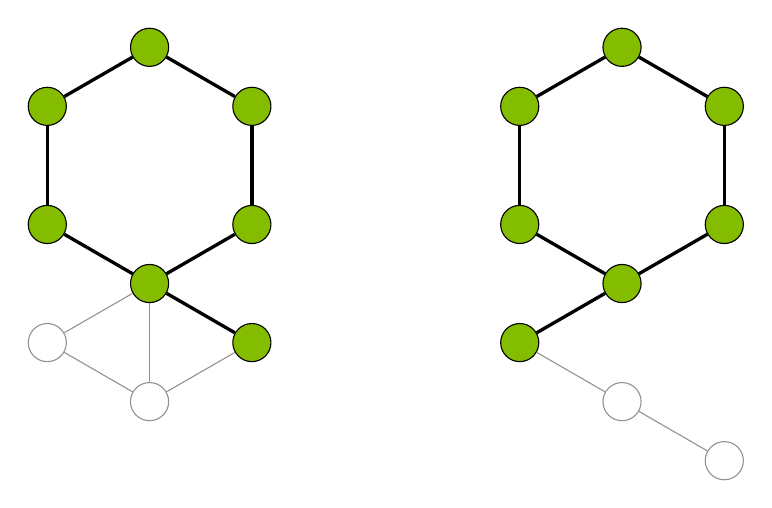
\begin{tikzpicture}
        \begin{scope}
            \node[draw, circle, fill=uofglawn, inner sep=2pt, font=\normalsize] (M1) at (90:1.5) {\phantom{0}};
            \node[draw, circle, fill=uofglawn, inner sep=2pt, font=\normalsize] (M2) at (150:1.5) {\phantom{0}};
            \node[draw, circle, fill=uofglawn, inner sep=2pt, font=\normalsize] (M3) at (30:1.5) {\phantom{0}};
            \node[draw, circle, fill=uofglawn, inner sep=2pt, font=\normalsize] (M4) at (210:1.5) {\phantom{0}};
            \node[draw, circle, fill=uofglawn, inner sep=2pt, font=\normalsize] (M5) at (330:1.5) {\phantom{0}};
            \node[draw, circle, fill=uofglawn, inner sep=2pt, font=\normalsize] (M6) at (270:1.5) {\phantom{0}};
            \node[draw, circle, draw=uofgsandstone!60, fill=white, inner sep=2pt, font=\normalsize] (M7) at ($(210:1.5) + (M6)$) {\phantom{0}};
            \node[draw, circle, fill=uofglawn, inner sep=2pt, font=\normalsize] (M8) at ($(330:1.5) + (M6)$) {\phantom{0}};
            \node[draw, circle, draw=uofgsandstone!60, fill=white, inner sep=2pt, font=\normalsize] (M9) at ($(270:1.5) + (M6)$) {\phantom{0}};

            \draw [very thick] (M1) -- (M2);
            \draw [very thick] (M2) -- (M4);
            \draw [very thick] (M3) -- (M5);
            \draw [very thick] (M4) -- (M6);
            \draw [very thick] (M5) -- (M6);
            \draw [very thick] (M3) -- (M1);
            \draw [color=uofgsandstone!60] (M6) -- (M7);
            \draw [very thick] (M6) -- (M8);
            \draw [color=uofgsandstone!60] (M6) -- (M9);
            \draw [color=uofgsandstone!60] (M7) -- (M9);
            \draw [color=uofgsandstone!60] (M8) -- (M9);
        \end{scope}

        \begin{scope}[xshift=6cm]
            \node[draw, circle, fill=uofglawn, inner sep=2pt, font=\normalsize] (M1) at (90:1.5) {\phantom{0}};
            \node[draw, circle, fill=uofglawn, inner sep=2pt, font=\normalsize] (M2) at (150:1.5) {\phantom{0}};
            \node[draw, circle, fill=uofglawn, inner sep=2pt, font=\normalsize] (M3) at (30:1.5) {\phantom{0}};
            \node[draw, circle, fill=uofglawn, inner sep=2pt, font=\normalsize] (M4) at (210:1.5) {\phantom{0}};
            \node[draw, circle, fill=uofglawn, inner sep=2pt, font=\normalsize] (M5) at (330:1.5) {\phantom{0}};
            \node[draw, circle, fill=uofglawn, inner sep=2pt, font=\normalsize] (M6) at (270:1.5) {\phantom{0}};
            \node[draw, circle, fill=uofglawn, inner sep=2pt, font=\normalsize] (M7) at ($(210:1.5) + (M6)$) {\phantom{0}};
            \node[draw, circle, draw=uofgsandstone!60, fill=white, inner sep=2pt, font=\normalsize] (M8) at ($(270:1.5) + (M6)$) {\phantom{0}};
            \node[draw, circle, draw=uofgsandstone!60, fill=white, inner sep=2pt, font=\normalsize] (M9) at ($(330:1.5) + (M8)$) {\phantom{0}};

            \draw [very thick] (M1) -- (M2);
            \draw [very thick] (M2) -- (M4);
            \draw [very thick] (M3) -- (M5);
            \draw [very thick] (M4) -- (M6);
            \draw [very thick] (M5) -- (M6);
            \draw [very thick] (M3) -- (M1);
            \draw [very thick] (M6) -- (M7);
            \draw [draw=uofgsandstone!60] (M7) -- (M8);
            \draw [draw=uofgsandstone!60] (M8) -- (M9);
        \end{scope}
    \end{tikzpicture}
\end{frame}

\begin{frame}{Connectedness as a Constraint}
\end{frame}

\begin{frame}{Connectedness via Restricted Branching}
\end{frame}

\begin{nearlyplainframe}[t]{Constraint, Branching, or Both?}
    \only<1>{
        \begin{center}
            \includegraphics*{gen-graph-connected-cumulative-cp.pdf}
        \end{center}
    }
    \only<2>{
        \begin{center}
            \includegraphics*{gen-graph-connected-heatmap-cp.pdf}
        \end{center}
    }
\end{nearlyplainframe}

\begin{frame}{Connectedness in Clique-Like Algorithms}
    \begin{itemize}
        \item Connectedness doesn't decompose cleanly into binary constraints, so we can't encode it
            as microstructure.
        \item On the other hand, we \emph{can} use restricted branching, if we give more information
            to the clique algorithm.
            \begin{itemize}
                \item Integrating this with the bound and ordering heuristic is horribly technical.
            \end{itemize}
    \end{itemize}
\end{frame}

\begin{nearlyplainframe}[t]{Which is Better Now?}
    \only<1>{
        \begin{center}
            \includegraphics*{gen-graph-connected-cumulative.pdf}
        \end{center}
    }

    \only<2>{
        \begin{center}
            \includegraphics*{gen-graph-connected-heatmap.pdf}
        \end{center}
    }
\end{nearlyplainframe}

\begin{frame}{Some Perspective}
    \begin{itemize}
        \item These instances are \emph{much} smaller than the ones we can solve for subgraph
            isomorphism (35 / 35 vertices versus 1,000 / 10,000 vertices).
    \end{itemize}
\end{frame}

\begin{frame}{Other Things}
    \begin{itemize}
        \item Parallelism?
            \begin{itemize}
                \item Decomposition EPS-style for MCS is reported to be not particularly wonderful,
                    and for clique it's a really bad idea.
                \item Dynamic decomposition for clique is well-studied and gives extremely good
                    speedups when done in a particular way (but has yet to be implemented beyond
                    shared memory).
            \end{itemize}
        \item I think we can improve the clique algorithm.
            \begin{itemize}
                \item The bound sometimes does silly things with association graphs.
                \item Can we do fancier or cheaper propagation?
                \item Better vertex ordering?
            \end{itemize}
        \item Other side constraints?
        \item Connectedness in directed graphs?
    \end{itemize}
\end{frame}

\begin{frame}[plain,noframenumbering]
    \begin{center}
        \vspace*{4em}
        \url{http://www.dcs.gla.ac.uk/~ciaran} \\
        \vspace{1em}
        \href{mailto:c.mccreesh.1@research.gla.ac.uk}{\nolinkurl{c.mccreesh.1@research.gla.ac.uk}} \\
    \end{center}

    \begin{tikzpicture}[remember picture, overlay]
        \node at (current page.north west) {
            \begin{tikzpicture}[remember picture, overlay]
                \fill [fill=uofguniversityblue, anchor=north west] (0, 0) rectangle (\paperwidth, -3.2cm);
            \end{tikzpicture}
        };
    \end{tikzpicture}
\end{frame}

\end{document}

